\chapter{CARBON MONOXIDE-INDUCED RESTRUCTURING ON PLATINUM (321), (112), (765), \& (557) SURFACES}
\label{chap:facet}
%\chapter{EFFECTS OF STEP-TYPE ON THE CO-INDUCED SURFACE RECONSTRUCTIONS OF PT(557)/(112)/(321)/(765) FACETS}

%\begin{abstract}
%The effects of step-edge type and plateau length on \ce{CO}-induced
%restructuring of \ce{Pt} were explored using molecular dynamics (MD)
%simulations. Platinum systems displaying four separate facets, [(321), (765),
%(112), (557)], were constructed and exposed to various coverages of carbon
%monoxide (\ce{CO}).  Platinum-\ce{CO} interactions were parameterized from
%experimental data and Density Functional Theory (DFT) calculations, providing
%classical potentials that capture the atop binding preference on \ce{Pt}. The
%differences in binding strength between edge atoms on the various facets were
%found to play a significant role in step-edge wandering and possible
%reconstruction events. Additionally, as the mechanism for step-edge doubling
%has been seen to depend on a stochastic process of two edges meeting, the
%varying sizes of the plateaus was also found to play a large role in these
%reconstructions.  The lack of observed step-doubling on the (557) surface
%throughout the simulation time suggests that this process is quite sensitive to
%the strength of \ce{CO} binding as well as being dependent on the initial
%random meeting of two separate edges.
%\end{abstract}
%\newpage


In this chapter we explore four facets of \ce{Pt} exposed to \ce{CO} through
molecular dynamics simulations. The facets were chosen to explore the effects
plateau length and step-edge, flat or kinked, have on previously identified
reconstruction processes. The rougher, {\em i.e.} kinked, (321) and (765)
systems might be expected to undergo greater amounts of step-wandering while
also experiencing step-edge doubling at a faster rate than the previously
modeled, flat (557) systems. The change in the local coordination environment was also
examined as the surfaces underwent reconstruction, as this is an important
descriptor of potential catalytic activity. 

%\section{Introduction}
%Industrial catalysts often consist of supported metal nanoparticles or
%high-index metal surfaces as both of these materials have a high density of
%low-coordinated atoms which have been shown to be active for catalyic
%reactions.\citep{Jeong:1999aa, Larsen:1999aa} Numerous studies have examined
%catalytic activity on low-energy metal surfaces, primarily the (111), (110),
%and (100) facets which are only somewhat applicable to industrial
%conditions.\citep{Stephens:2011bv, Stamenkovic:2007kk, Mohsenzadeh:2015kx,
%?,?,?,?} However, because of the advent of High Pressure Scanning Tunneling
%Microscopy (HP-STM) and Ambient Pressure X-ray Photoelectron spectroscopy
%(AP-XPS), these systems can now be explored at higher temperatures and
%pressures which allows for a better understanding of the surface structures of
%industrial catalysts.  These roughened surfaces and nanoparticles are of
%particular interest because their predicted morphology and stability at high
%temperatures and pressures has been seen to strongly depend on the presence and
%identity of adsorbates.\citep{Tao:2008aa, Tao:2010aa, Tao:2011aa, Kim:2016cr,
%Eren:2016qt, Michalka:2013aa, Michalka:2015aa} That is, under reaction
%conditions, many of these catalysts have been observed to reconstruct, which
%can drastically change the surface of the catalyst leading to likely changes in
%the activity and selectivity of the material.
%
%One system that has received significant attention is the \ce{Pt} (557) surface
%exposed to \ce{CO}. Tao {\em et al.} using HP-STM, AP-XPS, and Density Functional
%Theory (DFT) calculations observed that by introducing carbon monoxide (\ce{CO}) to
%the system, the stepped Pt surface would undergo a step-doubling reconstruction resulting in
%step-edges that were twice as high and plateaus that were twice as long as on
%the original surface.\citep{Tao:2010aa} If the system was maintained at these conditions, the
%appearance of triangular nanoclusters bridging the steps were also eventually
%observed. After removing \ce{CO} from the system, it was found that
%these changes were reversible as the \ce{Pt} (557) surface was recovered.  It was
%suggested that this reconstruction was caused by the repulsive forces between
%adsorbed \ce{CO} molecules.  This system was also explored with molecular
%dynamics simulations and a possible mechanism to explain the step-doubling was
%proposed which also strongly depended on the \ce{CO}-\ce{CO} quadrupolar
%repulsion.\citep{Michalka:2013aa}
%
%The strong interaction of \ce{CO} with \ce{Pt} has been explored on different
%systems and similar results have been observed. Ferrer {\em et al.} examining
%\ce{Pt} (997) observed both \ce{O} and \ce{CO} induced step-doubling on the
%surface. They also saw that the presence of step-doubling was correlated with a
%factor of three increase for \ce{CO} oxidation.\citep{Balmes:2016uf} Park {\em
%et al.}, again exploring the \ce{Pt} (557) system exposed to \ce{CO}, saw that
%the ordering of the triangular nanoclusters is very sensitive to temperature
%and can undergo its own reversible restructuring separate from the doubling
%already observed on this surface.\citep{Kim:2016cr} Moving away from \ce{Pt},
%Eren {\em et al.} found that a flat (111) \ce{Cu} surface when exposed to
%\ce{CO} also underwent reconstruction, forming small nanoclusters on the
%surface that were highly active for the oxygen reduction reaction
%(ORR).\citep{Eren:2016qt} In all of these cases, the presence of adsorbates led
%to large-scale reconstructions (often reversible) of the system, however, the
%specifics of the dynamics are still being explored.
%
%Continuing in this vein, this paper examines the effect of carbon monoxide on
%various platinum facets, specifically focusing on the effect of step-type and
%plateau length. The \ce{Pt} (321) \citep{Mcclellan:1981aa, Bray:2014aa,
%Bray:2011aa}, \ce{Pt} (112) \citep{Xu:1995aa, Yates:1995aa}, \ce{Pt} (765), and
%\ce{Pt} (557) \citep{Michalka:2015aa, Michalka:2013aa, Tao:2010aa, Kim:1997aa}
%systems were chosen as they represent a mix of flat and kinked edges as well as
%short and long plateau lengths. Based on the proposed mechanism in reference
%\citenum{Michalka:2013aa}, it is hypothesized that the length of the plateau
%and the roughness of the step edge will both strongly contribute to whether
%reconstruction will occur on these surfaces.  These systems were modeled using
%classical force fields that balanced maximizing chemical accuracy, while
%simultaneously minimizing computational time.  The use of  molecular dynamics
%methods was necessary to observe the assumed long-time dynamics of these large
%systems which when previously investigated were on the order of 10s-100s of
%nanoseconds.

\section{Methodology}
Platinum-platinum interactions were modeled with the Embedded-Atom-Method (EAM)
which is described more fully in Chapters \ref{chap:intro} and
\ref{chap:island}.\citep{Foiles:1986ky}

%Modeling the surface reconstruction of a solid/gas interface requires large
%systems.  To observe events such as step doubling and step wandering, systems
%need to contain on the order of 10\textsuperscript{3} - 10\textsuperscript{4}
%atoms. The large number of electrons involved with this many atoms means that
%these interfaces cannot be modeled through ab {\em ab initio} molecular
%dynamics (AIMD),\citep{Kresse:1993ve, Kresse:1993qf, Kresse:1994ul}
%Car-Parrinello methods, \citep{Car:1985bh, Izvekov:2000fv, Guidelli:2000fy} or
%quantum mechanical potential energy surfaces.  In addition, the interactions
%between the individual metal atoms is poorly represented by classical pairwise
%interactions.  Therefore, the Embedded Atom Method (EAM) \citep{Foiles:1986ky}
%was used to model the \ce{Pt\bond{-}Pt} interactions.  The molecular model for
%carbon monoxide (\ce{CO}) was developed by Straub and
%Karplus,\citep{Straub:1991no} and it treats the \ce{CO} as a rigid, three-site
%body. It was chosen primarily because it describes \ce{CO}'s strong linear
%quadrupole accurately.  The \ce{Pt\bond{-}CO} interaction was modeled to match
%a combination of experimental \citep{Ertl:1977cg, Kelemen:1979ad, Yeo:1997th}
%and theoretical \citep{Feibelman:2001qa, Deshlahra:2009wu, Beurden:2002ys,
%Deshlahra:2012aa, Korzeniewski:1986kl, Mason:2004ix} data. 
%
%\subsection{Platinum-Platinum interactions}
%Since classical force fields often do not work well for transition metal
%systems, several methods have been developed that use a non-pairwise additive
%function of the local electron density.  Some of these methods include the
%embedded atom method (EAM) \citep{Foiles:1986ky, Daw:1984aq, Johnson:1989yr,
%Daw:1989ci, Plimpton:1993qi, Voter:1995ax, Lu:1997fv, Alemany:1998fp}, the
%Finnis-Sinclair method \citep{Finnis:1984hl, Sutton:1990rr} and the
%quantum-corrected Sutton Chen method \citep{Qi:1999dn}.  In general, these
%methods treat the atom as a positive core surrounded by a radially decaying
%negative charge density due to valence electrons.  The energy necessary to
%place a core at location $i$ requires knowing the electron density, $\rho_i$,
%at that point as contributed by all other metallic atoms in the system and is
%represented below, 
%
%\begin{equation}
%\rho_{i} = \sum_{j \ne i}\rho_{j}(\mathbf{r}_{ij})
%\end{equation}
%
%In the equation above, $\rho_{j}(\mathbf{r}_{ij})$ describes how the valence
%electron distribution of atom $j$ varies with the radius.  The potential from
%embedding the atom $i$ at the location in question becomes
%
%\begin{equation}
%V_{i} = F[\rho_{i}] + \sum_{j \ne i} \phi_{ij}(\mathbf{r}_{ij})
%\end{equation}
%
%In equation (2), $F[\rho_{i}]$ is a functional which describes the primarily
%attractive force between the positive core and the electron density surrounding
%the other atoms while $\phi_{ij}(\mathbf{r}_{ij})$ represents the pair-wise
%repulsion between the positively charged cores.  Potentials similar to the ones
%shown above are used in the EAM, Finnis-Sinclair, and the Quantum Sutton Chen
%methods.  These methods have been used for a variety of purposes such as
%examining bulk and nanoparticle properties, \citep{Chui:2003fk, Wang:2005qy,
%Medasani:2007uq, Mishin:1999ew} melting,\citep{Belonoshko:2000jk,
%Sankaranarayanan:2006ye, Sankaranarayanan:2005bh} fracture,
%\citep{Shastry:1996qg, Shastry:1998dx, Mishin:2001qt} crack propagation,
%\citep{Becquart:1993sr} and alloying dynamics.  \citep{Shibata:2002hh,
%Mishin:2002if, Zope:2003ai, Mishin:2005vc} EAM's parameterization included
%second and third nearest-neighbor interactions which makes it particularly
%suited to systems that are expected to deviate from low-energy (111) surfaces,
%which is why it was chosen to describe the \ce{Pt\bond{-}Pt} interactions of
%our high-index surfaces.  \citep{Foiles:1986ky} 

\subsection{Carbon Monoxide model}
The carbon monoxide model developed by Karplus and Straub\citep{Straub:1991no},
which was discussed in Chapter \ref{chap:PtAu} and shown in Table \ref{tab:CO}
is used here without change.
%The large linear quadrupole moment of \ce{CO} is believed to play a primary
%role in the reconstruction of \ce{Pt} (557)\citep{Tao:2010aa, Michalka:2013aa}
%and since Karplus and Straub's model captures that quadrupole it was chosen for
%this work.\citep{Straub:1991no} This model consists of three rigid sites, 2
%atomic describing the \ce{C} and \ce{O} both with an attached negative charge
%and a massless site at the center of mass that carries a large positive charge.
%The necessary parameters are shown in Table \ref{tab:parameters}.  These
%parameters still produce a small dipole moment of 0.35 D while keeping the
%linear quadrupole (-2.40 D\AA) close to both experiment (-2.63 D\AA)
%\citep{Chetty:2011dp} and quantum mechanical predictions (-2.46 D\AA).
%\citep{Rizzo:2000sp}

%\begin{table}
%\caption{PARAMETERS FOR THE CO MODEL}
%%\caption{Positions, Lennard-Jones parameters ($\sigma$ and $\epsilon$) and charges for \ce{CO\bond{-}CO} interactions}
%\centering
%\begin{threeparttable}
%\centering
%\begin{tabular}{c c c c c}
%\hline
%\hline
% & z \tnote{a} & $\sigma$ \tnote{a} & $\epsilon$ \tnote{b} & q \tnote{c}\\
% \hline
% C & -0.6457 & 3.83 & 0.0262 & -0.75 \\
% O & 0.4843 & 3.12 & 0.1591 & -0.85 \\
% M & 0.0 & & & 1.6 \\
%\hline
%\hline
% \end{tabular}
%\begin{tablenotes}
%  \item \ce{CO\bond{-}CO} cross-interactions are modeled with Lennard-Jones potentials.
%  \item[a] Positions are given in \AA
%  \item[b] Energies are given in kcal/mol
%  \item[c] Charges are given in elementary units, $e^{-}$
%\end{tablenotes}
%\end{threeparttable}
%\label{tab:parameters}
%\end{table}

\subsection{Platinum-Carbon Monoxide interactions} The extensive experimental
\citep{Ertl:1977cg, Kelemen:1979ad, Yeo:1997th, Szanyi:1992aa, Schweizer:1989fk, Ertl:1989}
and theoretical \citep{Feibelman:2001qa, Deshlahra:2009wu,
Deshlahra:2012aa, Beurden:2002ys, Korzeniewski:1986kl, Mason:2004ix} work on
\ce{Pt\bond{-}CO} allows for significant data upon which to parameterize this
interaction.  The \ce{Pt\bond{-}CO} interaction has been
modified from previous models\citep{Michalka:2013aa, Michalka:2015aa} to better
capture the difference in energy between the preferred atop and bridge sites as
described by DFT calculations.\citep{Deshlahra:2012aa} The model has also been
modified to use a purely repulsive Morse potential to represent the
\ce{Pt\bond{-}O} interaction in contrast with previous
implementations.\citep{Korzeniewski:1986kl, Michalka:2013aa} Using a purely
repulsive Morse prevents unphysical \ce{O} binding to the surface.
Combining the Lennard-Jones \ce{Pt\bond{-}C} interaction with the repulsive
Morse describing the \ce{Pt\bond{-}O} interaction, provides the following
potential form for the \ce{Pt\bond{-}CO} interaction,

\begin{equation}
V_{r} = 4\epsilon\bigg(\Big(\frac{\sigma}{r_{Pt-C}}\Big)^{12} - \Big(\frac{\sigma}{r_{Pt-C}}\Big)^{6}\bigg) + D_{e}e^{-2\gamma(r_{Pt-O}-r_{e})}
\end{equation}

Table \ref{table:pt-co} shows the parameters for the above potential, while
Table \ref{table:sites} provides the binding energies for the various sites
based on these parameters and compares them to DFT\citep{Deshlahra:2012aa} and
experimental data.\citep{Ertl:1977cg, Kelemen:1979ad}

\begin{table}
\caption{REFIT PARAMETERS FOR THE PT-CO CROSS-INTERACTIONS}
%\caption{Parameters for Pt-CO Interaction}
\centering
\begin{threeparttable}
\centering
\begin{tabular}{c c c c c}
\hline
\hline
\multicolumn{2}{c}{Pt-C} & \multicolumn{3}{c}{Pt-O}  \\
\hline
$\sigma$\tnote{a} & $\epsilon$\tnote{b} & $r_{e}$\tnote{a} & $\mathrm{D}_e$\tnote{b} & $\gamma$\tnote{c} \\
\hline
1.68 & 52.25 & 5.15 & 0.03 & 1.7 \\
\hline
\hline
\end{tabular}
\begin{tablenotes}
  \item Metal-C interactions are modeled with Lennard-Jones potentials, while the metal-O interactions were fit to Morse potentials.
  \item[a] Distances are given in \AA
  \item[b] Energies are given in kcal/mol
  \item[c] $\gamma$ is given in units of \AA\textsuperscript{-1}
\end{tablenotes}
\end{threeparttable}
\label{table:pt-co}
\end{table}

\begin{table}
\caption{ADSORPTION ENERGIES FOR CO ON PT(111) WITH NEW PARAMETERIZATION}
%\caption{Pt-CO Binding Site Preferences (eV)}
\centering
\begin{threeparttable}
\centering
\begin{tabular}{c c c c}
\hline
\hline
& Atop & Bridge & Hollow \\
\hline
This work & -1.49 & -1.36 & -1.32 \\
DFT\tnote{a} & -1.48 & -1.47 & -1.45 \\
Experimental\tnote{b} & -1.43 & & \\
\hline
\hline
\end{tabular}
\begin{tablenotes}
  \item All binding energies are given in eV.
  \item[a] Ref. \citep{Deshlahra:2012aa}
  \item[b] Refs. \citep{Ertl:1977cg, Kelemen:1979ad}
\end{tablenotes}
\end{threeparttable}
\label{table:sites}
\end{table}


\subsection{Systems}

The stepped \ce{Pt} systems were created so as to be of a similar size, and fit
properly in an orthorhombic periodic box. The four surface cuts were doubled
in either the $x$ or the $y$ direction so that the effect of step lengths could
also be investigated and were identified as LS, for systems with longer steps,
and MS, for systems with more steps. The system dimensions, number of atoms,
and surface coverages are enumerated in Table \ref{tab:dimensions}. Each system
began as a FCC crystal and was cut to expose the desired face in the extended
$z$ axis, while staying periodic along the $x$ and $y$ axis.
%the pt(112) systems were
%8 layers thick, had a slab thickness of $\sim$18 \aa~and were in boxes of 65.70
%x 54.24 x 100 \aa~and 32.82 x 108.4 x 100 \aa.  the pt(557)
%systems were 10 layers thick, had a slab thickness of $\sim$21 \aa~ and were in
%boxes of 55.27 x 49.48 x 100.3 \aa~and a 110.6 x 24.76 x 100.3
%\aa.  the pt(321) systems were 8 layers thick, had a slab thickness of
%$\sim$18 \aa~and were in boxes of 35.82 x 95.49 x 100 \aa~and 71.70 x
%47.71 x 100 \aa. the pt(765) systems were 9 layers thick, had a slab
%thickness of $\sim$19 \aa~and were in boxes of 58.36 x 50.19 x 100 \aa~
%and 28.72 x 100.5 x 100 \aa.  

\begin{table}
\caption{SYSTEM DIMENSIONS FOR THE STEPPED PT SURFACES}
%\caption{Dimensions}
\centering
\begin{threeparttable}
\centering
\begin{tabular}{c c c c c}
\hline\hline
Surface & Atoms & Surface Atoms & \multicolumn{2}{c}{System dimensions\tnote{a} (MS \& LS)}  \\ 
\hline
(321) & 4440 & 720 & 71.7 x 47.7 x 100 & 35.8 x 95.5 x 100  \\
(112) & 4608 & 768 & 32.9 x 108.5 x 100 & 65.8 x 54.3 x 100 \\
(765) & 3744 & 792 & 28.7 x 100.5 x 100 & 58.4 x 50.2 x 100 \\
(557) & 3888 & 720 & 110.6 x 24.8 x 100 & 55.3 x 49.5 x 100 \\
\hline
\hline
\end{tabular}
\begin{tablenotes}
  \item Systems were replicated in either the $x$ or $y$ dimension at the
beginning of the simulations to examine the effect of edge length and quantity
of steps on the reconstruction process.
  \item[a] Box dimensions are given in \AA
\end{tablenotes}
\end{threeparttable}
\label{tab:dimensions}
\end{table}

The systems were then run in the canonical (NVT) ensemble, gradually raising
the temperature to either 700\ ~K or 1000\ ~K depending on the initial
stability of the pure system.  The systems with longer plateaus were more
stable and were run at 1000\ ~K to bring reconstruction dynamics into the
domain of typical simulation times.  Gas phase CO molecules, corresponding to
0.25 ML or 0.5 ML of surface coverage were placed in the vacuum region and then
allowed to adsorb on the surface. The systems were then re-equilibrated for
approximately one nanosecond before data collection was begun.  Data was
collected by running the systems in the microcanonical (NVE) ensemble for 100
ns.  Simulations were performed using the open source molecular dynamics
package, OpenMD.\citep{Fennell:2006xq, Meineke:2005pt, openmd} 

\section{Results}

%\subsection{Diffusion}
%Make a table... hopefully the burrowing will explain most of this
%Additionally, when double steps (or partial double steps form) there is not as much movement afterwards, so that is a possible explanation as well
% Try to show a count of mobile atoms (as a function of time maybe)

\subsection{Generalized coordination number}
Many catalytic reactions have a degree of structural sensitivity such that only
a subset of the displayed atoms on a roughened surface or nanoparticle are
actually catalytically active. While the coordination number of individual
atoms can help describe their binding strengths, Calle-Vallejo {\it et al.}
have observed that including the first and second nearest neighbor counts in
their description of coordination allowed for a better description of an atom's
local environment.\citep{Calle-Vallejo:2015qq} With this information 
they were able to create ``coordination-activity plots'' that
related an atoms coordination with its catalytic activity, similar to volcano plots. Since they needed to
include information about second nearest neighbors, they introduced a new term,
the generalized coordination number (GCN) as a useful measure of the various
binding environments on metal surfaces or nanoparticles. 

\begin{equation}
  \overline{CN}(i) = \sum_{j=1}^{n_i}\frac{cn(j)}{cn_{\textrm{max}}}
  \label{eq:gcn}
\end{equation}

The GCN is a straight-forward extension of a nearest-neighbor analysis with the
primary difference being that the GCN of an atom $i$, $\overline{CN}(i)$,  is
calculated from the average of the coordination numbers, $cn(j)/cn_\textrm{max}$,
of its nearest neighbors.  The sum is over atom $i$'s first nearest neighbors
and $cn_\textrm{max}$ is a normalization term and for an FCC crystal is equal
to 12, the bulk coordination number.

\begin{figure}[p!]
  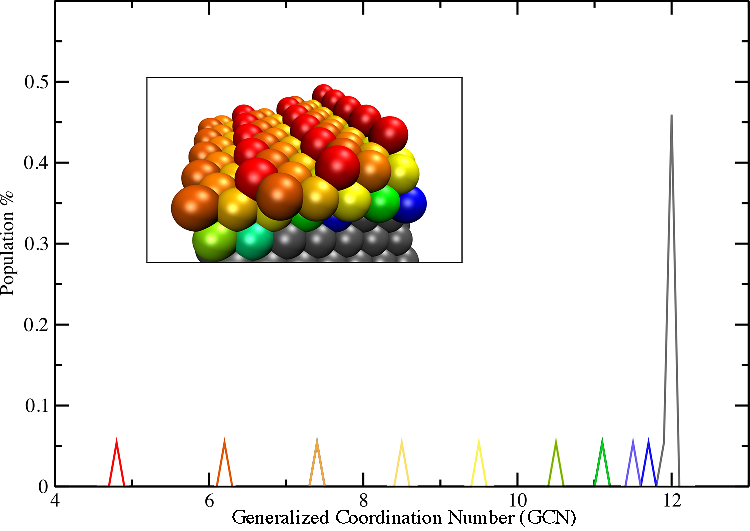
\includegraphics[width=\linewidth]{../figures/chap4/321_ideal_gcn.pdf}
  \caption{A graph of the generalized coordination number of an ideal Pt (321)
system colored to match the inset figure. Other than the bulk (GCN = 12), the
ideal (321) surface displays a wide variety of environments for its surface
atoms.  The edge atoms (red) have the lowest GCN because they are 
under-coordinated, whereas the plateau atoms have GCN's around the ideal
surface number of 7.5. Subsurface atoms (yellow, greens, and blues) have a
larger GCN then the surface, but are still less than the bulk GCN of 12.  }
\label{fig:ideal321GCN}
\end{figure}

The concept is further illustrated in Figure \ref{fig:ideal321GCN} where we see
an ideal \ce{Pt} (321) surface color coded to match the encompassing GCN graph.
The bulk atoms (GCN=12) make up the majority of the system, however, there is a
wide range of potentially catalytically active sites on the surface.
Specifically, Calle-Vallejo {\em et al.} argued that for the Oxygen Reduction
Reaction (ORR) a \ce{Pt} atom with a GCN of $\sim$8.3 would be the most
catalytically active site. Since an ideal (111) surface in composed of atoms
with a GCN of $7.5=(6\times9 + 3\times12)/12$, this implies that surfaces that
display some amount of concavity may be necessary to achieve the highest
catalytic activities. Another color-coded graph of an ideal \ce{Pt} (557)
system is included in Appendix \ref{app:SI2} as Figure \ref{fig:557GCN} to
highlight the differences between a rough surface, (321), to a comparatively
flat surface, (557).

In Figure \ref{fig:LS321GCNF}, we see GCN data from the \ce{Pt} (321) systems
which are focused on the surface and subsurface layers, i.e. non-bulk, for the
three examined coverages at  the beginning and end of the simulation times. The
growth in the peaks around 7.5, as highlighted with the blue bar, suggest that
the surface is reconstructing, displaying larger (111) domains. The amount of
CO present in the system plays a direct role in this reconstruction.
Additionally, the decrease in peaks at 4.5 and 6.2 provide evidence of the
system moving to a lower energy facet.  The growth in the peak at a GCN of 11.2
shows how the subsurface layers are becoming more bulk-like.

\begin{figure}[p!]
  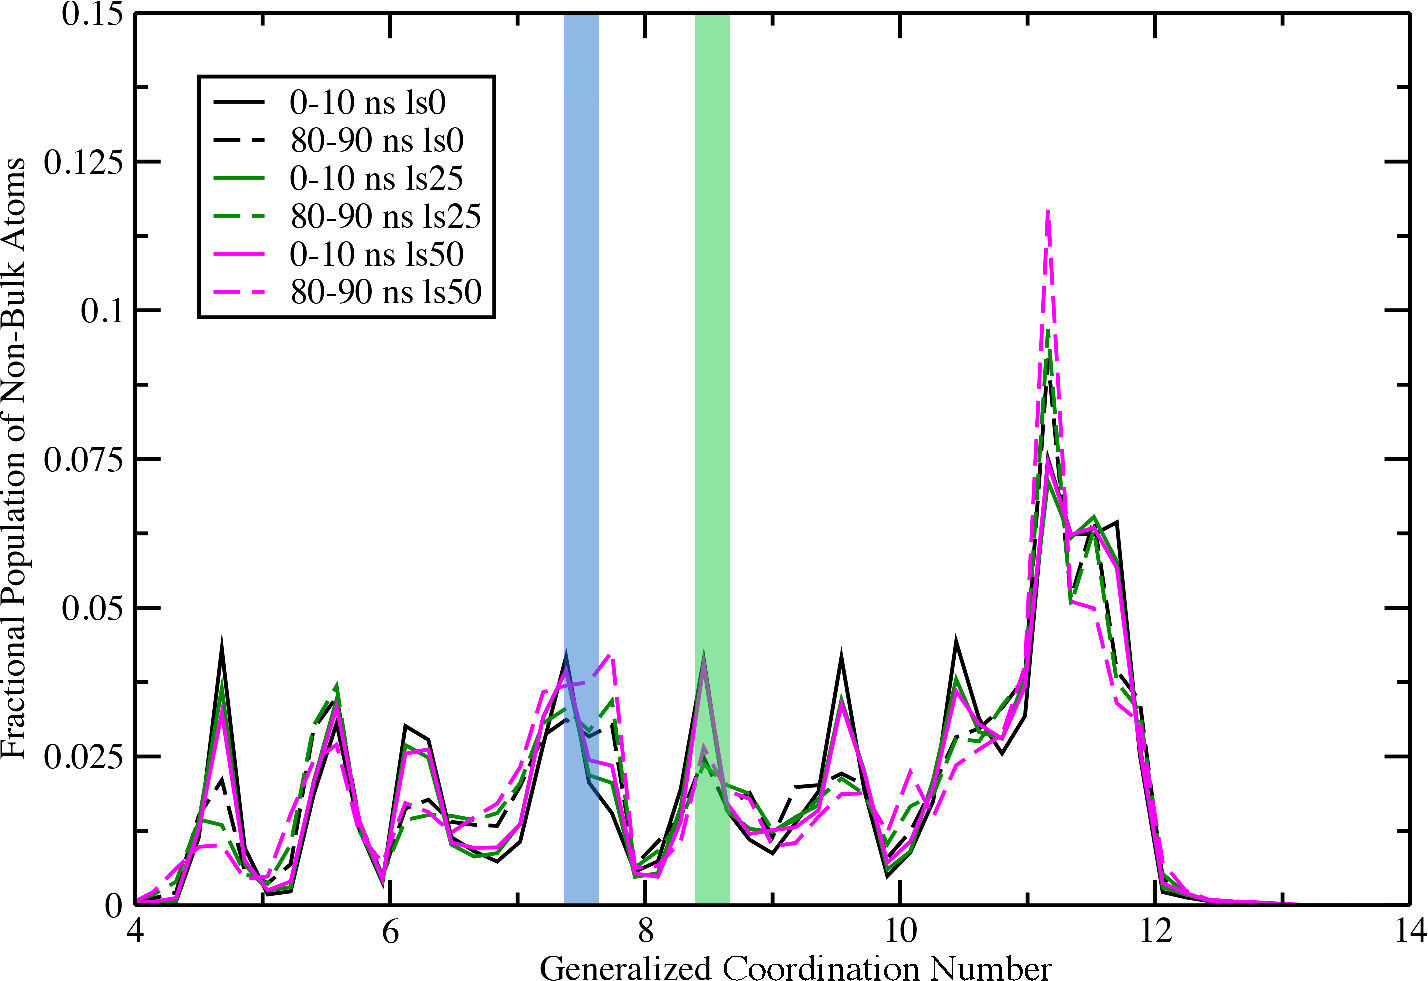
\includegraphics[width=\linewidth]{../figures/chap4/321ls_GCNF.pdf}
  \caption{Plots of the average GCN for the non-bulk atoms of the \ce{Pt} (321)
LS systems.  Solid lines represent the averaged GCN during the first 10
nanoseconds of simulation time, while the dotted lines correspond to a time near
the end of the simulations. Black lines indicate the bare 0 ML system, while
green and magenta depict the 0.25 ML and 0.5 ML systems respectively. The blue
bar is aligned at a GCN=7.5 which corresponds to the GCN of a surface atom in
an ideal \ce{Pt} (111) surface, while the green bar highlights the region
identified by Calle-Vallejo {\em et al.} as being especially active for ORR
activity.\citep{Calle-Vallejo:2015qq}}
\label{fig:LS321GCNF}
\end{figure}

The other systems examined in this study experienced much less reconstruction,
as evidenced in their GCN plots. Figure \ref{fig:LS112GCNF} shows the
calculated GCN's of the \ce{Pt} (112) LS systems and the minimal changes that
the system exhibited during the simulation. There is a slight reduction of
population around 5.5 which is consistent with the step sinking that was
observed on some of these systems. Representative GCN plots of the other
systems are included in Appendix \ref{app:SI2} as Figures \ref{fig:557lsGCN}
through \ref{fig:765lsGCN}.

\begin{figure}[p!]
  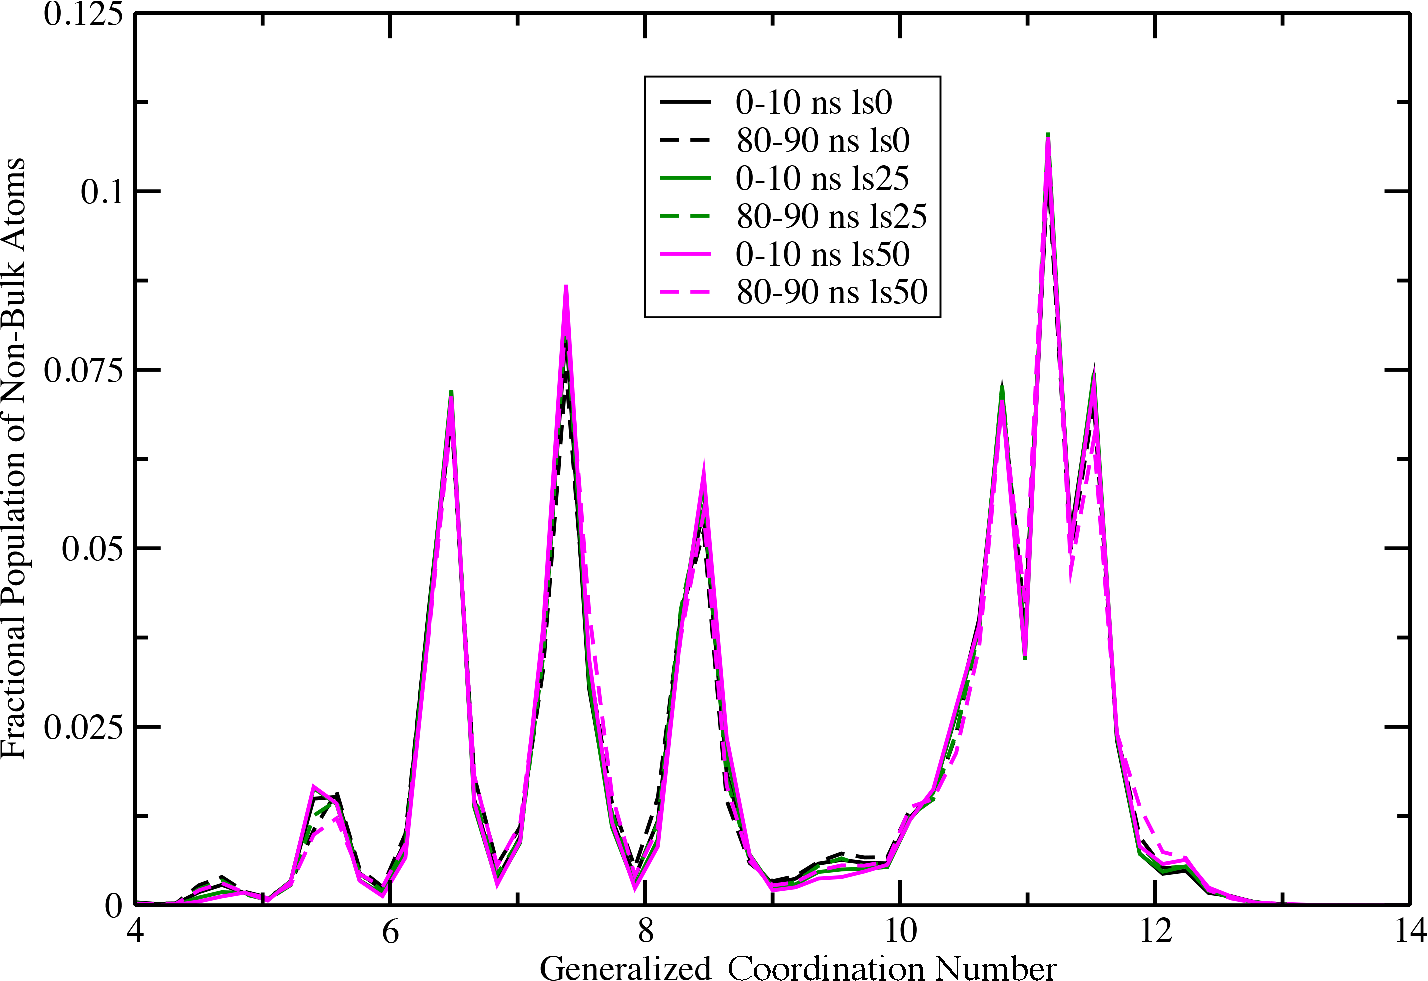
\includegraphics[width=\linewidth]{../figures/chap4/112ls_GCNF.pdf}
  \caption{Plots of the average GCN for the non-bulk atoms of the Pt (112) LS
systems. Solid lines represent the averaged GCN during the first 10 nanoseconds
of simulation time, while the dotted lines correspond to a time near the end of
the simulations. Black, green and magenta lines depict the 0, 0.25, and 0.5 ML
systems respectively. Except for a slight shrinking of the peak at 5.5 combined
with some growth at 9.5 and around 12, the local environment of this system is
barely perturbed.}
\label{fig:LS112GCNF}
\end{figure}

\subsection{Edge wandering}
All of the surfaces experienced some amount of step-wandering which will be
discussed by facet below.

\subsubsection{Pt (557)}
The (557) surfaces have been explored more fully in previous
papers,\citep{Tao:2010aa, Michalka:2013aa}, but we must  report that no
doubling was observed during the simulation time despite the large degree of
step wandering. The two most likely explanations include the stochastic nature
of this reconstruction. Additionally, the \ce{Pt\bond{-}CO} interaction has
been weakened compared to the fit in the previous paper.\citep{Michalka:2013aa}
It is likely that both of these explanations are contributing factors as there
was significant step-wandering, but the key event (two step-edges meeting) did
not occur for any of the (557) systems simulated in this study.

\subsubsection{Pt (112)}
The (112) MS surfaces exhibited restructuring to relieve residual surface tension.
This resulted in a number of the
originally (100) step edges sinking into the surface and shifting
sideways to display a sunken (111) step edge. This is highlighted in Figure
\ref{fig:112sunken} in Appendix \ref{app:SI2}.  Adatom formation from these (111)
steps was minimal and the total amount of adatom creation and movement on
these systems was much less than on the (112) systems with longer steps. 

The (112) LS surfaces exhibited moderate step-wandering, although limited
step-edge reconstructions were observed. Some of the steps on each system sunk
into the bulk, making adatom formation difficult.  The bare surface maintained
its displayed (112) step-edges macroscopically.  We also observed that there
was significant adatom ejection and re-adsorption on the surface. The presence
of \ce{CO} increased the disruption of the step-edges and the largest amount of
restructuring in these systems was observed on the 0.5 ML system.  Three steps
in this system coalesced into a mini-(111) facet, highlighted in Figure
\ref{fig:tripleStep}.

\begin{figure}
\centering
  \includegraphics[width=0.8\linewidth]{../figures/chap4/112_tripleStep.pdf}
  \caption{Top-down view of the (112) 0.5 ML surface extended to display longer
steps. (a) depicts the system at the beginning of the run when minimal
step-wandering had occurred. (b) Near the end of the simulation, three edges
had begun to coalesce into a triple step, highlighted in yellow.}
  \label{fig:tripleStep}
\end{figure}

\subsubsection{Pt (765)}
The (765) surfaces, while undergoing significant amounts of step-wandering did
not experience any clear instances of step-edge doubling during the
simulations. The MS systems, those extended to display more steps, maintained
the (765) motif over the entire simulation (barring one incident on the 0.5 ML
system). What appears to be the initial stages of a doubling event results in
portions of both involved edges sinking into the surface of the metal. This
process is shown in Figure \ref{fig:765Edge} in Appendix \ref{app:SI2}.

The LS systems also experienced significant step-wandering. While no doubling
was observed, connections between separate edges were seen. However, these
connections led to some of the steps rotating on the surface of the metal.
Despite the apparent stability of the (765) motif for the MS systems, the 0 and
0.5 ML LS systems appeared to undergo an unstructured reconstruction that lead
to an increase of the GCN at 6.8 highlighted in Figure \ref{fig:765lsGCN}.

\subsubsection{Pt (321)}
The (321) steps showed the most interesting behavior. Numerous instances of
step doubling were observed on both the MS and LS 0.5 ML systems. The 0.25 ML
systems also showed minor reconstruction, although little doubling
was observed. The 0 ML systems did experience a small amount of step-wandering,
likely due to the high energy of the surface and the elevated temperatures the
systems were run at.

An interesting case of frustrated double layer formation is highlighted in
Figure \ref{fig:partialDoubleLayer} where three double layers have begun to
form, but the center double layer highlighted in green is preventing the blue
or red double layer from coalescing. Within our simulation time, the 0.5 ML
LS systems were not observed to form a double step that encompassed the length
of the system, whereas numerous examples of partial double steps can be found.

\begin{figure}
\centering
\includegraphics[width=\linewidth]{../figures/chap4/321_partialDoubleLayer.pdf}
\caption{Images of the (321) 0.5 ML LS systems at the (a) beginning and
(b) end of the simulation time. Before \ce{CO} is added to the system the
kinked edges are well maintained barring slight dislocations. After a
significant amount of simulation time, \ce{CO} induced double step formation.
The plateaus are sufficiently narrow that the initial step of this process, forming a
``nucleation'' site can happen numerous times between separate steps.
Highlighted in (b) are frustrated double layers, where any ``zippering'' that
would be expected to finish the formation of a double layer is hindered by the
resultant un-zippering of another layer.}
\label{fig:partialDoubleLayer}
\end{figure}

While there was a significant amount of step-wandering observed on the (321)
0.25 LS surface, the system appeared to get trapped in a meta-stable state
highlighted in Figure \ref{fig:diamonds}. There is a small amount of step-edge
doubling in these systems, but the majority of the system is taken up by small
diamond shaped (111) domains. The formation of so many nucleation sites between
step edges may suggest a possible reason for the pausing at this configuration
and will be explored in more detail in the discussion.

\begin{figure}
\centering
\includegraphics[width=\linewidth]{../figures/chap4/321MiniDiamonds.pdf}
\caption{The (321) 0.25 ML LS system at the (a) beginning and (b) end of the
simulation. The red outline highlights one of the repeated (111) ``diamond''
domains formed between the initially regular steps.}
\label{fig:diamonds}
\end{figure}

\section{Discussion}
Based on the results of our previous work\citep{Michalka:2013aa}, we predicted
that all of these systems would have a high likelihood of undergoing
double-layer reconstruction. While the amount of step-wandering was significant
for the majority of the systems exposed to \ce{CO}, only the (321) surfaces
demonstrated repeated step-edge doubling. One explanation for this surprising
result is that our modification of the \ce{Pt\bond{-}CO} forcefield to bring it
closer to experimental results weakened the \ce{Pt\bond{-}CO} step energetics
in these systems. Here we will discuss the features of the forcefield and the
studied systems while also examining the effects of step type and plateau
length on step-wandering.

\subsection{Surface energy}
Surface energies were calculated for every system that was studied, as well as
for the low-index Pt(111), Pt(100), and Pt(110) surfaces.  To perform these
calculations, systems were created such that they were periodic in all
directions ({\em x, y, z}). The desired surface was then exposed by extending
the box size in the {\em z}-direction sufficiently to prevent long-distance
interactions between steps.  The change in the potential energy that resulted
was used to calculate the surface energy.  The values calculated for the
low-energy surfaces matched previous values calculated using EAM, which is
expected as they were one of many experimental variables that were used to
parameterize the EAM forcefields.\citep{Foiles:1986ky} These values differ
slightly from experimental\citep{Tyson:1977xe, De-Boer:1988tg, Galeev:1980pt} and
DFT\citep{Vitos:1998qq} sources, but match in terms of ratios between the
various surfaces.  The surface energies of Pt(111), Pt(110), and Pt(100) that
were calculated in this experiment are compared to those calculated in previous
EAM experimentation \citep{Foiles:1986ky} as well as against experimental
surface energy values in Table \ref{table:lit_surface_energy}.

\begin{table}
\caption{SURFACE ENERGY VERIFICATION OF LOW-INDEX PT SURFACES}
%\caption{Surface Energy Verification}
\centering
\begin{threeparttable}
\centering
\begin{tabular}{c c c c c }
\hline
\hline
Facet & Surface Energy & EAM\tnote{a} & Experimental\tnote{b} & Sim./Exp.\\
\hline
\ce{Pt} (111) & 1.43 & 1.44 & 0.977 & 1.46 \\
\ce{Pt} (100) & 1.63 & 1.65 & 1.286 & 1.27 \\
\ce{Pt} (110) & 1.75 & 1.75 & 1.553 & 1.13 \\
\hline
\hline
\end{tabular}
\begin{tablenotes}
  \item All energies are given in J/$\textrm{m}^2$
  \item[a] Ref. \citep{Foiles:1986ky}
  \item[b] Ref. \citep{Galeev:1980pt}
\end{tablenotes}
\end{threeparttable}
\label{table:lit_surface_energy}
\end{table}

The same methodology was used to calculate surface energies for the \ce{Pt}
(765), \ce{Pt} (557), \ce{Pt} (112), and \ce{Pt} (321) surfaces and these energies are shown
in Table \ref{table:surface_energy}.  The surface energy of these systems is
inversely correlated to the distance between step-edges. This is reasonable as
the larger step length corresponds to a larger amount of the low-energy (111)
facet being displayed. This suggests that the higher surface energy systems
will be more amendable to reconstruction as they can then display a greater
proportion of (111) domains.

\begin{table}
\caption{SURFACE ENERGY AND STEP-LENGTH CALCULATIONS FOR MODELED PT SURFACES}
%\caption{Surface Energy}
\centering
\begin{threeparttable}
\centering
\begin{tabular}{c c c}
\hline
\hline
Facet & Surface Energy\tnote{a} & Step Separation\tnote{b} \\
\hline
%pt(765) & 1.525686968 & 16.79333333 \\
%pt(557) & 1.546605208 & 13.785 \\
%pt(112) & 1.673338459 & 6.79 \\
%pt(321) & 1.756522657 & 5.901440476 \\
\ce{Pt} (765) & 1.53 & 16.79 \\
\ce{Pt} (557) & 1.55 & 13.79 \\
\ce{Pt} (112) & 1.67 & 6.79 \\
\ce{Pt} (321) & 1.76 & 5.90 \\
\hline
\hline
\end{tabular}
\begin{tablenotes}
  \item[a] Energies are given in J/$\textrm{m}^2$
  \item[b] Distances are given in \AA
\end{tablenotes}
\end{threeparttable}
\label{table:surface_energy}
\end{table}

\subsubsection{Plateau length}
In addition to the plateau length providing a good measure of the surface
energy of these facets, the length of the plateau also plays a role in the
mechanism of restructuring. The mechanism for doubling as proposed in reference
\citep{Michalka:2013aa} and mentioned previously, is strongly dependent on
two step-edges meeting and forming a stable nucleation site from which a
``zippering'' process can speed up the rest of the reconstruction. As the
meeting of two step-edges is primarily a stochastic process, anything that
makes the initial meeting less likely, like increasing the distance between
steps, will make the reconstruction process more difficult to capture with our
finite simulation times. This combined with the retuning of the
\ce{Pt\bond{-}CO} forcefield, explains why despite seeing significant
step-wandering on the (557) and (765) systems little to no reconstruction was
observed during the 100 ns of simulation, whereas the (321) surfaces exhibited 
many doubling events. This would suggest that the (112) surface should also
have seen significant doubling, and while there was one instance of a triple
step beginning to form, the slight reconstruction that sunk a number of the
step-edges made any sort of adatom formation on those surfaces difficult.
Recreating the (112) systems and relieving residual surface tension 
would likely lead to a larger amount of step doubling.

\subsection{Energy to separate from edge}
As the formation of adatoms is essential for step-wandering and step-doubling,
energy curves describing this process were computed for several \ce{CO}
configurations, as had been done previously.  \citep{Michalka:2013aa,
Michalka:2015aa} These calculations were performed at various displacements as
the atoms of interest were moved perpendicular to the step edge along the
plateau as shown in Figures \ref{fig:112_557_ES} and \ref{fig:321_765_ES}. The
strong quadrupolar repulsion between aligned \ce{CO} leads to this process of
adatom formation becoming energetically favorable at high coverages. For the
faceted (112) and (557) systems, configurations e, g, and h, highlighted in
Figure \ref{fig:112_557_ES}, make the initial formation of an adatom an
energetically favorable process. The (321) and (765) facets examined in Figure
\ref{fig:321_765_ES}, owing primarily to their rougher step edges, show that
configurations e, f, g, and h are all favorable for adatom formation.

\begin{landscape}
\begin{figure}[p!]
  \centering
  \includegraphics[width=0.9\linewidth]{../figures/chap4/112_557_EnergySeparation_CO.pdf}
  \caption{Energies for displacing an edge atom (*) perpendicularly from the
step edge. The top and bottom graphs contain data for the (112) and (557)
surfaces, respectively.  Each of the energy curves corresponds to one of the
labeled configuration on the right and are referenced to the unperturbed step
edge. The spheres represent Pt atoms on the upper (white) and lower (grey)
steps.  Colored atoms (blue) are depicted with a CO molecule adsorbed in an
atop configuration. Certain configurations of CO, notably g and h, can lower
the energetic barrier for creating an adatom.}
\label{fig:112_557_ES}
\end{figure}
\end{landscape}

\begin{landscape}
\begin{figure}[p!]
  \centering
  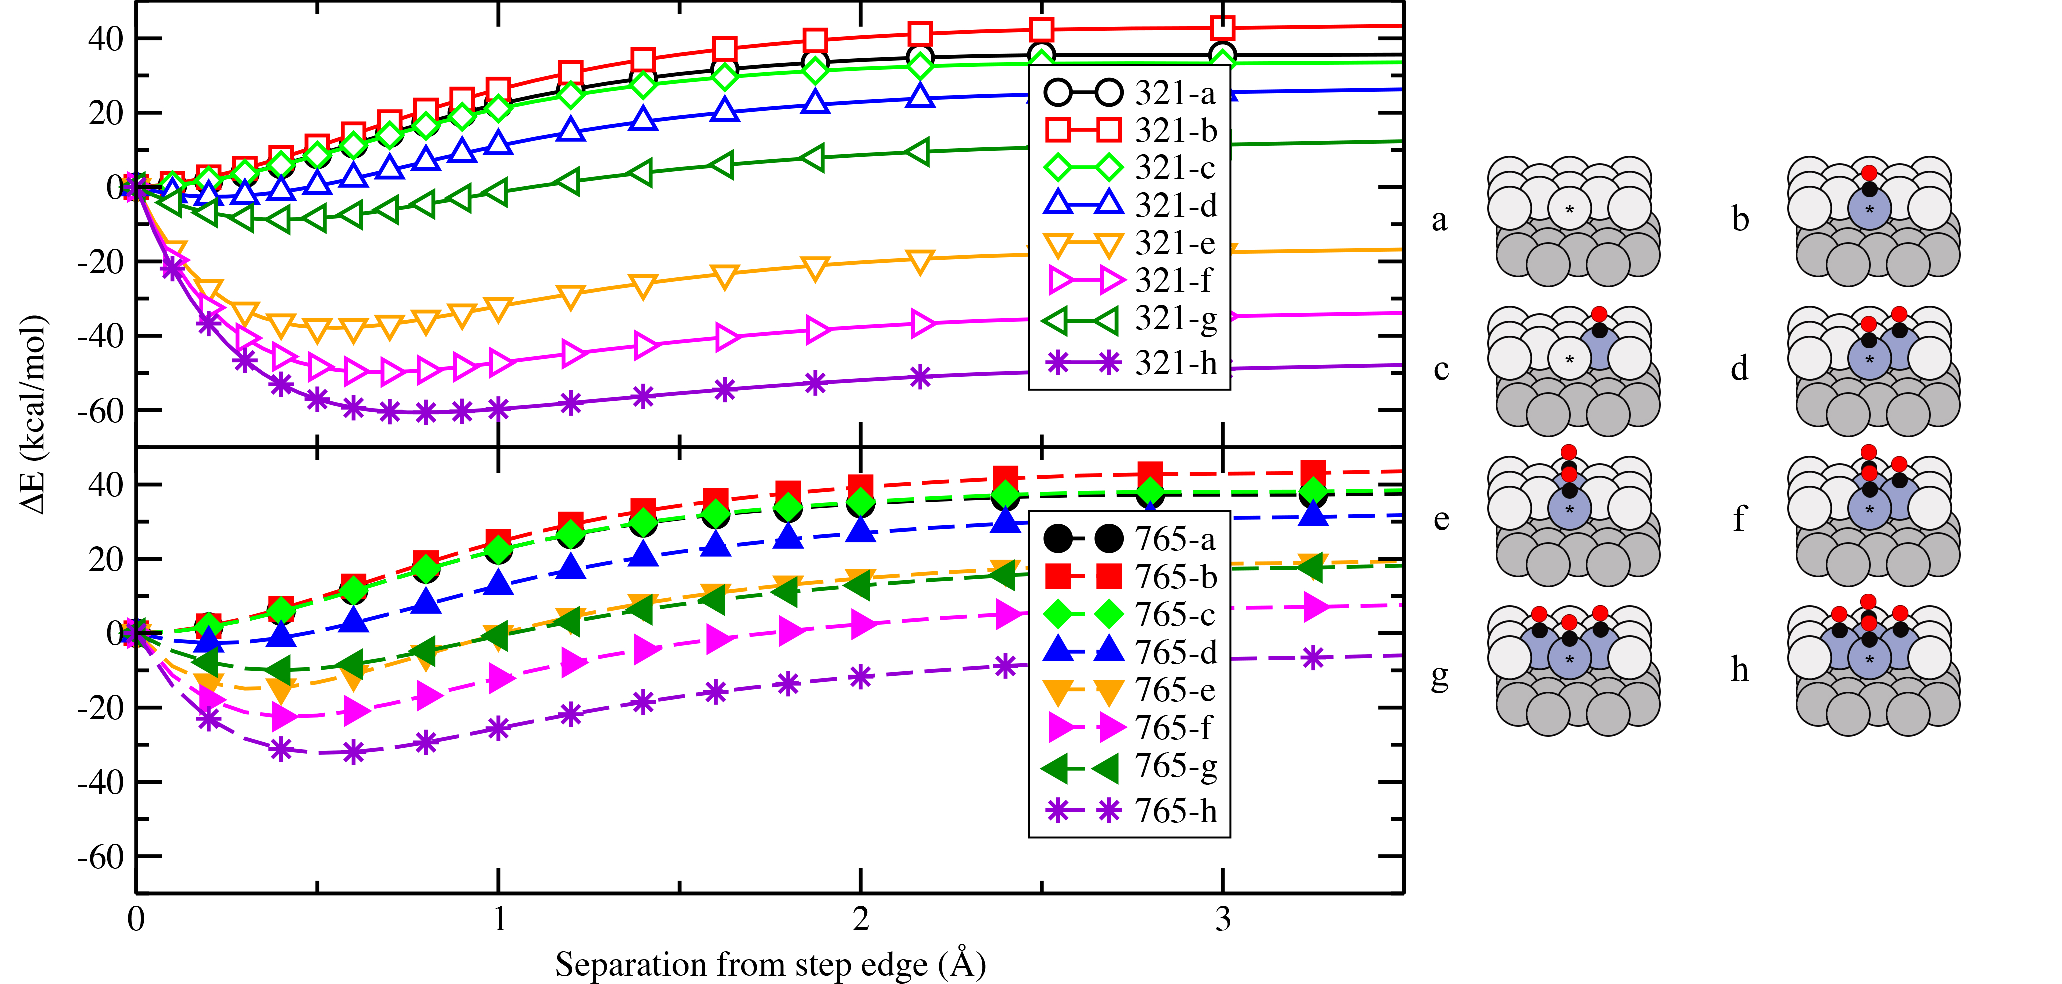
\includegraphics[width=0.9\linewidth]{../figures/chap4/321_765_EnergySeparation_CO.pdf}
  \caption{Similar to Figure \ref{fig:112_557_ES}, these graphs depict the
energies for displacing an edge atom perpendicularly from either the (321) or
(765) step edges. The configurations to the right of the graphs represent the
rougher kinked step edges of these facets. The rougher steps lower the 
energetic barrier for adatom creation when compared to the flat steps of the
(112) and (557) surfaces.}
\label{fig:321_765_ES}
\end{figure}
\end{landscape}

In general, this analysis provides several helpful results. First, removing an
atom from a (321) or (765) step is more energetically favorable than from a
(112) or (557) step. This is due to the lower coordination of atoms in
the kinked edges. This trend is clearly shown in Figures \ref{fig:112_557_ES}
and \ref{fig:321_765_ES} for configuration {\em a} where no CO is present on the
surface. In these instances, removing an atom from a kinked step edge is 10
kcal/mol more favorable than it is to form an adatom from a flat step. This is
due to the lower coordination of the atoms in the kink steps.
Additionally9, the length of the plateau seems to also affect the energy required to form
an adatom at higher coverages.  Configurations e, f, and h in Figure
\ref{fig:321_765_ES} for the kinked steps highlights this result well. It is
approximately 25 kcal/mol more favorable to form an adatom on the (321) surface
than it is on the (765) surface. Similarly, there is approximately a 20
kcal/mol difference in favor of forming  forming an adatom from a (112) step-edge when
compared to the (557) surface.

Finally, the location and arrangement of \ce{CO} also strongly affects the
required energy to remove the atom from the step edge. Separation becomes most
favorable when the atom that is becoming the adatom and the atom directly
behind it both have an adsorbed \ce{CO}. This configuration directs the strong
quadrupolar repulsive force directly away from the step edge, thus lowering the
energetic barrier for adatom formation.  This conclusion can be demonstrated by
comparing configurations d and e in both figures. In configuration e, the
\ce{CO} are located along a vector which is aimed perpendicularly away from the
step, while in configuration d the repulsive force generated by the \ce{CO} is
mostly parallel to the step edge. As the coverage
increases, the likelihood of a higher energy configuration also increases,
which leads to more step-edge breakup and a larger surface diffusion.

\subsubsection{Straight vs. Kinked edges}
As highlighted in Figure \ref{fig:diamonds}, one of the partial reconstructions
observed on the (321) surface are the small diamonds composed of (111) domains
formed between steps. Most of these diamonds share corners corresponding to
nucleation sites between steps from which zippering into double steps is
observed primarily on the 0.5 ML surfaces. The initial formation of these
diamonds however is of fairly low cost. Principally, the hopping
diagrammed in Figure \ref{fig:kinkSketch} has a barrier of approximately 40
kcal/mole in the worst case, while the resulting structure is within 0.1 kcal/mole of the original
surface. Since the presence of \ce{CO} provides some of the driving force for
this hopping, the resultant increase in (111) domain size on the surface
combined with the numerous nucleation sites that are formed between steps leads
to this patterning existing as a metastable state in many of our simulations of
the (321) surface. In contrast, the straight steps on the (112) and (557)
surfaces, while sources for adatoms, did not provide any benefit to doubling.

\begin{figure}
  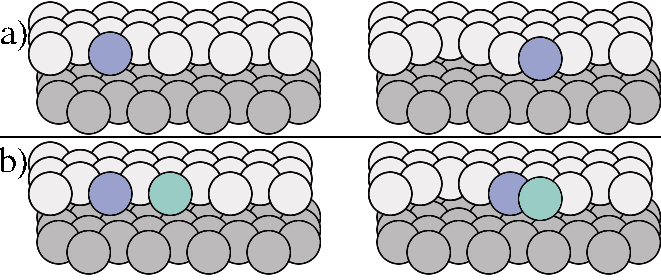
\includegraphics[width=\linewidth]{../figures/chap4/kinkMovement.pdf}
  \caption{Models of the ``kinked'' edge features of the (321) and (765)
surfaces.  One of the most commonly observed adatom movements on the surface
involves one of the kink atoms hopping to a nearby edge binding site. This is
predicted to happen in one of two ways, (a) the highlighted blue atom is
ejected and traverses in a curvilinear path to its end point or (b) the blue
atom dislocates the green atom resulting in the same final configuration. The
formation of longer (100) segments of the step-edge slightly lowers the surface
energy leading to a more stable surface.}
  \label{fig:kinkSketch}
\end{figure}

\subsection{CO binding energy}
%Coverage, temperature of system (compare to original data?)
The decrease in the parameterized \ce{Pt\bond{-}CO} interaction was made in
response to recent DFT results\citep{Deshlahra:2012aa} and uncertainties about
previously reported calorimetric heats of adsorption for the \ce{Pt\bond{-}CO}
interaction.\citep{Yeo:1997th} As the decrease in this binding energy results
in fewer CO being adsorbed at any given instant in the simulations, this also
leads to a decrease in adatom generation and concomitantly a decrease in
step-edge wandering. For the surfaces that had short plateaus, this decrease
did not appear to affect the doubling as the edges did not have to wander as
far to still meet, but for the (557) and (765) surfaces,  doubling was not
observed for this parameter set.

\subsection{Mechanisms of structural changes}
Our previous work on \ce{Pt} (557) revealed that the presence of \ce{CO} initially
destabilizes the step-edges leading to rapid formation of adatoms and
step-wandering on the surface. If significant step-wandering occurs such that
two edges connect, they often form a ``nucleation'' site, a location that
connects two step edges and is stable for a significant portion of time. Once
one of these sites is formed, step-wandering will often lead to ``zippering''
of the two edges into a double step. 

This mechanism initially depends on the stochastic meeting of two step edges
which is well-correlated with the density of adatom formation. Increased
thermal energy is one method to increase the number of adatoms on stepped
surfaces, however is these simulations we attempted to limit this through
lowered simulation temperatures.  The presence of \ce{CO} is playing a similar
role to an increased temperature by weakening the \ce{Pt\bond{-}Pt} bonds in
the step-edge.

The density of adatoms is one factor in determining the likelihood of step-edge
meeting, while the other primary factor is that of plateau length. The (112)
and (321) systems have shorter plateau lengths which makes the chance of
step-edges meeting more likely.  In our previous work on the (557) surface,
only one nucleation site formed per observed step-edge doubling, for some of
the systems explored in this study, numerous nucleation sites were created
before the steps could finish doubling, which in some cases led to partially
doubled step edges, highlighted in Figure \ref{fig:partialDoubleLayer}.

Further evidence of the importance of plateau length was elucidated from the
observed differences between the different (321), LS and MS, systems. The
longer steps tended to have more partially formed double layers as
a result of numerous nucleation sites. This prevented the full
zippering mechanism from occurring. In contrast, the (321) steps that were
extended to display a greater number of steps had a few
instances of complete step edge doubling.

All of the (321) surfaces, even those without \ce{CO} present showed some amount of surface
roughening and reconstruction suggesting that these surfaces are only quasi-stable
at high temperatures. However, the presence of \ce{CO} at 0.25 and 0.5 ML
coverages did lead to significantly more step-wandering intermediate
reconstructions and partial and full double layer formation.
%Dynamics of GCN for surfaces
%The slight refaceting of the surfaces led to an artificially low diffusion
%constant for these systems (true?) because the majority of steps have become
%slightly buried in these systems to reduce the high surface energy of these
%systems. Nevertheless, the remaining (100) steps were large sources of adatoms
%which was increased as \ce{CO} coverage was also increased. If the system were
%kept at an elevated pressure and prevented from relaxing along the
%step-direction, it is likely that the (100) steps would be better maintained
%and a larger amount of surface movement and eventual doubling would be
%observed.

\section{Summary}
The mechanism of reconstructions on \ce{Pt} surfaces, specifically step-edge
doubling, is dependent on the displayed surface facet. It is also
partially dependent on the presence of adsorbates, here \ce{CO}, that can 
disrupt the step-edges and then stabilize the formation of double steps. An in-depth
examination of the energetics of step-edge breakup shows that the ``kinked''
surfaces (321) and (765) are especially favorable for formation of adatoms
because of the under-coordination of the kinked edge atoms. The stochastic
mechanism proposed in earlier work which stated that the meeting up of two
edges was ultimately a stochastic process and then double layer formation would
typically proceed in a ``zippering'' fashion is strengthened here as a number of
systems with shorter plateaus ended up in frustrated double layer formations.

The lack of any double steps forming on the (557) surface despite being seen in
an earlier set of simulations suggests that the re-parameterization of the
\ce{Pt\bond{-}CO} interaction to better match reported experimental values has
altered the dynamics of the step-doubling process.  While significant
step-wandering was still observed on these systems, the density of adatoms was
not sufficient to stochastically form a nucleation site during the simulation
time.

Recent work on \ce{CO}-induced nanostructure formation on a \ce{Cu} (111) has
shown that when the metal-metal binding interactions are weaker, the presence
of strong repulsive adsorbates can be sufficient to disrupt even flat
surfaces.\citep{Eren:2016qt} We have reached a similar conclusion with the
\ce{Pt} systems explored for this investigation, such that surfaces that have a
higher surface energy and more sites where adatoms can be easily formed, ({\em
i.e.} weakly-bonded atoms) are more likely to experience reconstruction in
general and doubling of the step-edges specifically as this greatly increases
the amount of the surface that is occupied by the more stable (111) domains.

